\begin{figure}[h]
\centering
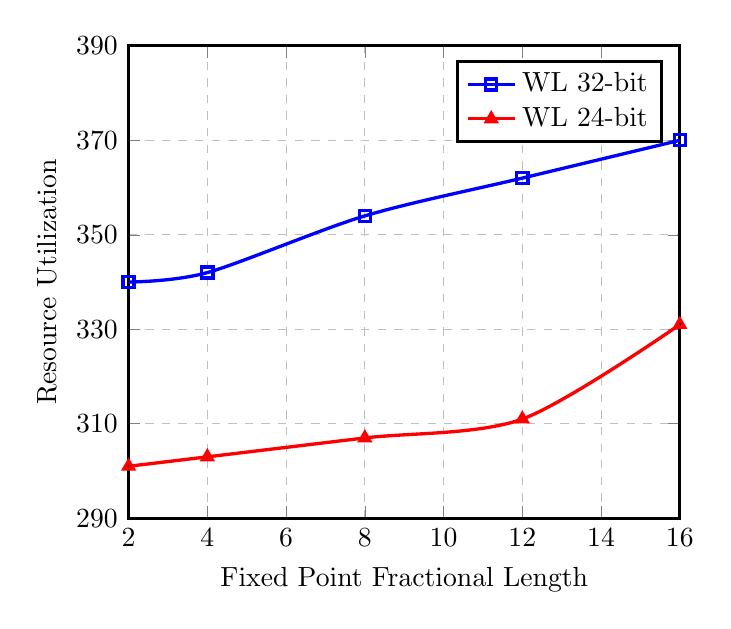
\begin{tikzpicture}
\begin{axis}[
scale only axis,
height=6cm,
width=7cm,
    xlabel={Fixed Point Fractional Length},
    ylabel={Resource Utilization},
    xmin=2, xmax=16,
    ymin=290, ymax=390,
    xtick={2,4,6,8,10,12,14,16},
    ytick={290,310,330,350,370,390},
    legend pos=north east,
    ymajorgrids=true,
    xmajorgrids=true,
    grid style=dashed,
    very thick
]
\addplot[
    color=blue,
    mark=square,
    smooth
    ]
    coordinates {
    (2,340)(4,342)(8,354)(12,362)(16,370)
    };
    \addlegendentry{WL 32-bit}
 \addplot[
    color=red,
    mark=triangle,
    smooth
    ]
    coordinates {
    (2,301)(4,303)(8,307)(12,311)(16,331)
    };
   \addlegendentry{WL 24-bit}
\end{axis}
\end{tikzpicture}
\caption{Effect of varying the Fractional Length on Resource Utilization}
\label{fig:5.5}
\end{figure}